\section{Greedy Algorithmen \tiny (Vorlesung 13 am 28.11.)}

\subsection{Intervallauswahl nach Endzeitpunkten}
Greedy-Algorithmus 
% Bild 1
\begin{figure}[h]
    \begin{center}
        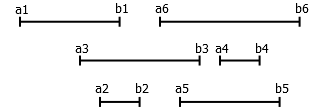
\includegraphics[width=\textwidth / 3]{../GFX/vl13_1.png}
        \label{fig:vl13_1}
    \end{center}
\end{figure}
%Alogrithmus Start
Sortiere die Intervalle nach Endzeitpunkt $b_1 \leq b_2 \leq ... \leq b_n$\\
r = $-\infty$
für $i = 1,...,n$\\ 
Wenn Intervalle $[a_i,b_i)$ keine ausgewähltes Intervall überlappt(\lstinline!if a_i \geq r!), wähle es aus (\lstinline!r = b_i!).\\
% Algorithmus Ende!
Wir müssen uns den rechtesten Punkt merken, um zur optimalen Lösung zu kommen...
$r$ = der rechte Endpunkt der bisher ausgewählten Intervalle.
\subsubsection{Beweis}
%Bild2
\begin{figure}[h]
    \begin{center}
        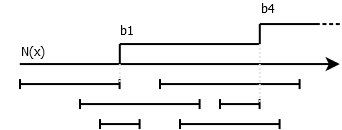
\includegraphics[width=\textwidth / 3]{../GFX/vl13_2.png}
        \label{fig:vl13_1}
    \end{center}
\end{figure}
$\mathcal{N}(x) = \#$der gewählten Intervalle innerhalb ($-\infty,x$) bei der Greedylösung.\\
$\mathcal{N}^*(x) = \#$der gewählten Intervalle bei einer beliebigen anderen Lösung.\\
Wir wollen zeigen, dass $\mathcal{N} \geq \mathcal{N}^*$ für alle $x$. $\mathcal{N}(\infty) \geq \mathcal{N}(\infty)$\\
$\mathcal{N}(x)$ kann sich nun an einem Punkt $b_i$ ändern.\\
Beweis mit Induktion nach $i$. $\mathcal{N}(b_i)\geq \mathcal{N}^*(b_i)$\\
Induktionsbehauptung: $\mathcal{N}(-\infty) = \mathcal{N}^*(-\infty) = 0$\\
Annahme: $\mathcal{N}^*(x)$ macht an der Stelle $b_i$ einen Sprung: $\mathcal{N}^*(b_i) = \mathcal{N}^*(b_{i-1})+1$.\\
Die andere Lösung wählt das Intervall $[a_i,b_i)$ aus.\\
$\mathcal{N}^*(b_i)  = \mathcal{N}^*(a_i)+1 \leq \mathcal{N}(a_i)+1$\\
Im Intervall $[a_i,b_i)$ hat der Greedy Algorithmus ebenfalls ein Intervall gewählt, das zu den bisherigen Intervallen disjunkt ist. (spätestens das Intervall $[a_i,b_i)$ ist so ein Kandidat. $\Rightarrow \mathcal{N}(b_i) \geq \mathcal{N}(a_i)+1 \leq \mathcal{N}(b_i)$ \\%Check!
Annahme (Fall2): $\mathcal{N}^*(x) $ macht keinen Sprung bei $b_i$\\%Check.

Im Vergleich zum Algorithmus der dynamischen Programmierung werden hier Vereinfachungen vorgenommen. 
\subsection{Variante}
Wir müssen alle Intervalle akzeptieren und sie verschiedenen Maschinen zuordnen, wenn sie sich überlappen.\\
Gesucht ist die minimale Anzahl von Maschinen.\\
% BILD IV ohne Nummern!
\begin{figure}[h]
    \begin{center}
        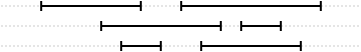
\includegraphics[width=\textwidth / 2]{../GFX/vl13_40.png}
        \label{fig:vl13_1}
    \end{center}
\end{figure}
Beispiel: Es sind 3 Maschinen notwendig.\\
Untere Schranke, Anzahl Intervalle die einem gemeinsamen Punkt $x$ enthalten.\\
\subsection{Greedy Algorithmus}
%algo start
Betrachte die Intervalle aufsteigend vom Startpunkt $a_1 \leq a_2 \leq ...\leq a_n$\\
Ordne jedes Intervall $[a_i,b_i)$ der Maschine mit der kleinsten Nummer $j$ zu, die frei ist.\\
%algo end
%Bild IV mit Nummern!
\begin{figure}[h]
    \begin{center}
        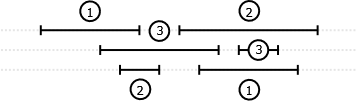
\includegraphics[width=\textwidth / 2]{../GFX/vl13_4.png}
        \label{fig:vl13_1}
    \end{center}
\end{figure}
\subsubsection{Beweis}
Behauptung: Wenn die Maschine $j$ zugeordnet wird, ist der Punkt $a_i$ in mindestens $j$ Intervallen enthalten.\\
Die Maschinen $1,2,...,j-1$ sind belegt und dabei in anderen Intervallen enthalten. plus Intervall $[a_i,b_i)$\\
\subsection{Interpretation als Graphenproblem}
Intervalle $\rightarrow$ Knoten\\
überlappende Intervalle $\rightarrow$ Kanten\\
%BILD 5
\begin{figure}[h]
    \begin{center}
        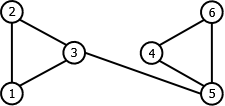
\includegraphics[width=\textwidth / 2]{../GFX/vl13_5.png}
        \label{fig:vl13_1}
    \end{center}
\end{figure}
Der entstehende Graph ist ein \underline{Intervallgraph}. Ein \underline{Durchschnittsgraph} von Intervallen.
% Exkurs Durchschnittsgraphen werden zum Beispiel im Mobilfunk verwendet, um Netzabdeckung optimal zu gestalten und Interferenzen zwischen zwei oder mehrere Sendemasten zu reduzieren.
Teilmenge von Intervallen, die sich nicht überlappen $\rightarrow$ unabhängige (Knoten-)Menge.\\
Überlappungsfreie Zuordnung von Maschinen $\rightarrow$ Graphenfärbung (chromatische Zahl $\psi$)\\
Punkt $x$, der in mehreren Intervallen enthalten ist $\rightarrow$ Clique. (vollständiger Teilgraph)\\
$\leftarrow$ gilt in Intervallgraphen aber nicht in allgemeinen Durchschnittsgraphen.\\
Die Cliquenzahl (Größe der größten Clique) nennen wir $\omega$\\
Ausserdem gilt für Intervallgraphen $\omega = \psi$ - sonst gilt im allgemeinen Durschnittsgraphen $\omega \leq \psi$\\

\subsection{Zeitplanung(Scheduling)}
Man hat $n$-Aufträge und jeder Auftrag hat eine Bearbeitungszeit $p_i$ und einen Termin $d_i$(deadline, due date) und die Aufträge müssen jetzt sequentiell abgearbeitet werden.\\
%Bild 6
\begin{figure}[h]
    \begin{center}
        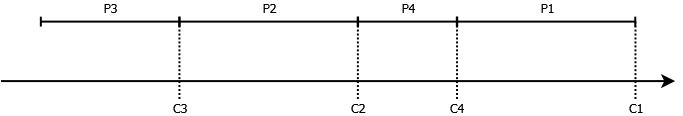
\includegraphics[width=\textwidth / 2]{../GFX/vl13_6.png}
        \label{fig:vl13_1}
    \end{center}
\end{figure}
Gesucht ist eine Reihenfolge in der die Aufträge bearbeitet werden.\\
Aus der Reihenfolge ergibt sich anschließend eine Abschlusszeit $C_i$, wann der Auftrag fertig ist.\\
Die Verspätung $L_i = \max \{C_i, d_i, 0\}$\\
Wir wollen die maximale Verspätung $\max\{L_i | i = 1,...,n\}$ minimieren.\\
Was passiert, wenn man zwei benachbarte Aufträge vertauscht. \\
% Bild 7
\begin{figure}[h]
    \begin{center}
        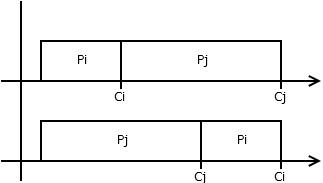
\includegraphics[width=\textwidth / 2]{../GFX/vl13_7.png}
        \label{fig:vl13_1}
    \end{center}
\end{figure}
Wir vergleichen: $\max\{C_j, C_i-d_i,0\}$\\
 $\max\{C'_j, C'_i-d_i,0\}$\\
 Es gilt: $C_j = C'_i > Ci,C'_j$\\
 Annahme, beide p's sind verspätet...
 %Bild 8
 \begin{figure}[h]
    \begin{center}
        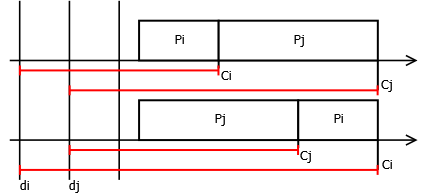
\includegraphics[width=\textwidth / 2]{../GFX/vl13_8.png}
        \label{fig:vl13_1}
    \end{center}
\end{figure}
 Behauptung: wenn $d_i \leq d_j$ ist, dann ist die Reihenfolge $ij$ mindestens so gut wie die Reihenfolge $ji$.\\
 $\max \{C_{max}-d_j,C_{i}-d_i\} \leq \max	\{C_{max}-d_i,C'_j-d_j\}$\\
 Wissen: $-d_j \leq -d_i$
 \subsubsection{Beweis}
 $C_{max}-d_j \leq C_{max}-d_i$\\
 $C_i - d_i \leq C_{max}-d_i$\\
 $\max \{C_{max}-d_j,C_i-d_i\} \leq C_{max} d_i \leq \max \{C_{max}-d_i,C'_j-d_j\}$\\
 \subsection{EDD-rule (earliest due date rule}
 Bearbeite die Aufträge in der Reihenfolge der Termine $d_i$.\\
 Beweis der Optimalität durch ein Austauschargument.\\
 
 \section{Der Klassiker für Greedy Algorithmen: minimal SPT}
 Gegeben ist ein zusammenhängender ungerichteter Graph mit Kantengewichten $\geq 0$.\\
 Gesucht ist ein Spannbaum, der alle Knoten enthält mit kleinstem Gesamtgewicht.\\
 Beispiel: siehe Bild:\\
 \begin{figure}[h]
    \begin{center}
        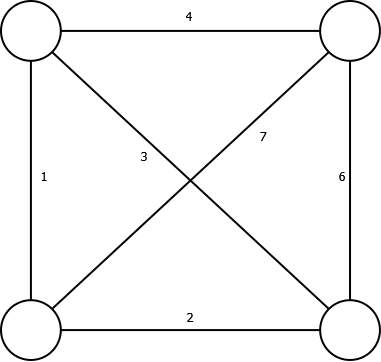
\includegraphics[width=\textwidth / 2]{../GFX/vl13_9.png}
        \label{fig:vl13_1}
    \end{center}
\end{figure}
 \subsection{Algorithmus von Kruskal}
 Betrachte die Kanten in der Reihenfolge nach Gewicht. Wähle die Kante aus, wenn sie mit den bisher gewählten Kanten keinen Kreis bildet.\\
 % 9 mit markierten Kanten!
 \begin{figure}[h]
    \begin{center}
        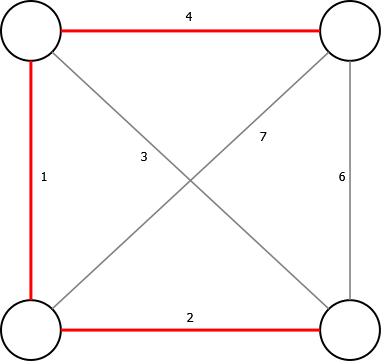
\includegraphics[width=\textwidth / 2]{../GFX/vl13_10.png}
        \label{fig:vl13_1}
    \end{center}
\end{figure}
Dieser Algorithmus hat zu einem grundlegenden Umdenken und weitreichenden Verallgemeinerungen geführt. Makroide. Wenn man eine beliebige Matrix nimmt und man betrachtet die unabhängigen Spaltenmengen, dann bilden die ein Makroid. Diese bilden dann eine Basis der Matrix.\\